\section{Durchführung}
\label{sec:Durchführung}

An den RLC-Schwingkreis wird mit einem Funktionsgenerator entsprechend Abblidung \ref{fig:Schaltung1}
eine Nadelimpulsspannung gegeben. Dabei wird der Strom über den Kreis mit dem kleinsten
Widerstand laufen gelassen. Mit einem Tastkopf wird die Spannung am Kondensator
abgegriffen und auf dem Bildschirm eines Oszilloskops ausgegeben. Bei hinreichend kleiner Frequenz der
Eingangsspannung lässt sich die Schwinung und das stetige Abfallen der Amplitude
der Kondensatorspannung beobachten. Mithilfe der Cursor-Funktion des Oszilloskops
werden daraus die Beträge der Amplitude zu unterschiedlichen Zeiten gemessen.

\begin{figure}[H]
  \centering
  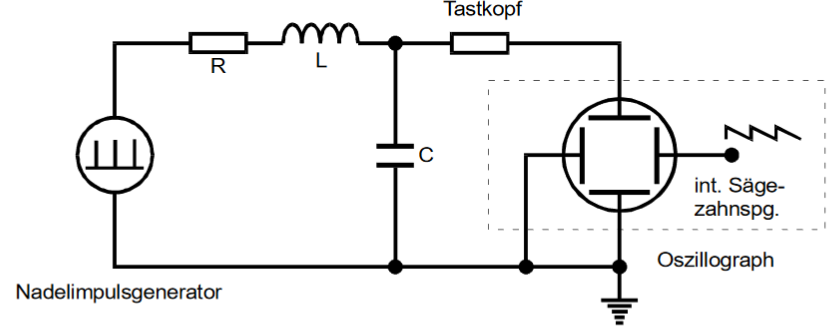
\includegraphics[width=14cm]{Schaltung1.PNG}
  \caption{Schaltung zur Messung der Kondensatorspannung. \cite{sample}}
  \label{fig:Schaltung1}
\end{figure}

Zur Bestimmung des Widerstands des aperiodischen Grenzfalls wird der Stromkreis
mit dem regelbaren Widerstand verwendet (Abbildung \ref{fig:Schaltung2}). Dieser wird solange variiert, bis die
Überschwingung der Kondensatorspannung gerade eben nicht mehr erkennbar ist.
Der zu diesem Zeitpunkt eingestellte Widerstand wird abgelesen.

\begin{figure}[H]
  \centering
  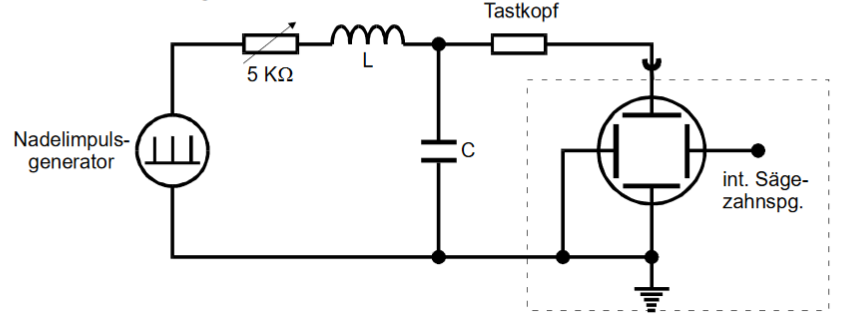
\includegraphics[width=14cm]{Schaltung2.PNG}
  \caption{Schaltung zur Messung des Widerstands des aperiodischen Grenzfalls. \cite{sample}}
  \label{fig:Schaltung2}
\end{figure}

Anschließend wird die Eingangsspannung auf eine Sinusspannung umgeschaltet und der Stromkreis mit dem größeren Widerstand verwendet
(Schaltung wieder wie in Abbildung \ref{fig:Schaltung1}).
Die Frequenz wird stückweise erhöht und die Kondensatorspannung in Abhängigkeit
der unterschiedlichen Frequenzen am Oszilloskop gemessen. Für die gleichen
Frequenzwerte wird im Anschluss die Amplitude der Eingangsspannung mit dem Tastkopf
gemessen da er einen eigenen Frequenzgang besitzt und seine Ausgangsspannung somit
nicht unabhängig von der Frequenz ist.

Um die Phasenverschiebung der Eingangs- und Kondensatorspannung zu messen,
lässt man beide Spannungen gegen die Zeit auf dem Bildschirm des Oszilloskops ausgeben (siehe Abbildung \ref{fig:Schaltung3}).
Die Frequenz der Eingangsspannung wird wieder stückweise erhöht. Dabei wird
die zeitliche Differenz der Maxima der angezeigten Spannungen (a) sowie die Periodendauer der Eingangsspannung (b)
gemessen (siehe Abbildung \ref{fig:Rechnung}).
Auch hier wird die Frequenz über drei Zehnerpotenzen hinweg erhöht.

\begin{figure}[H]
  \centering
  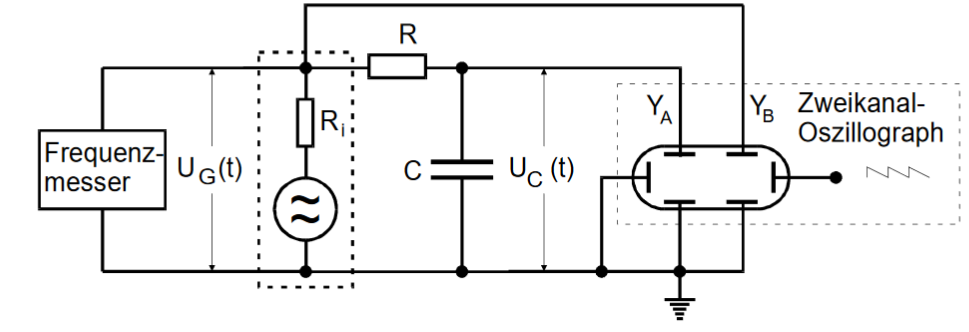
\includegraphics[width=14cm]{Schaltung3.PNG}
  \caption{Schaltung zur Messung der Phasenverschiebung der Spannungen. \cite{sample}}
  \label{fig:Schaltung3}
\end{figure}

\begin{figure}[H]
  \centering
  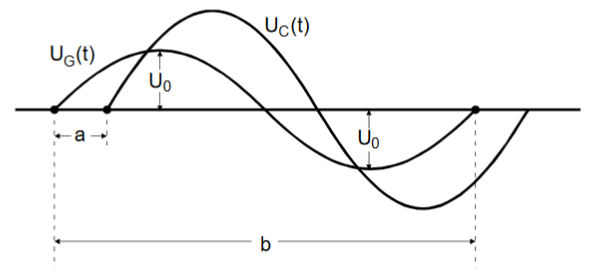
\includegraphics[width=14cm]{Rechnung.PNG}
  \caption{Berechnung der Phasenverschiebung. \cite{sample2}}
  \label{fig:Rechnung}
\end{figure}
